\documentclass[a4paper,11pt,titlepage]{article}
\usepackage[T1]{fontenc}
\usepackage[utf8]{inputenc}
\usepackage{lmodern}
\usepackage{array}
\usepackage{longtable}
\usepackage[english]{babel}
\usepackage{amsmath}
\usepackage{setspace}
\usepackage{changepage}
\usepackage{mathtools}
\usepackage[sorting=nyt,backend=bibtex,citestyle=authoryear]{biblatex}
\DeclarePairedDelimiter{\ceil}{\lceil}{\rceil}
\DeclarePairedDelimiter\abs{\lvert}{\rvert}
\newcommand{\norm}[1]{\left\lVert#1\right\rVert}
\usepackage{cancel}
\usepackage{amssymb}
\usepackage{graphicx}
\usepackage[colorlinks=true,linkcolor=blue]{hyperref}

\begin{document}

\section{Large d strategy}
For large d, we decided that we needed to design our strategy to optimize 
\begin{enumerate}
\item Total score by using as large a dance area as possible
\item Distribute this score across all players
\item Minimize number of moves required to distribute this score
\end{enumerate}

We discussed several different strategies to do these, one of which we agreed to implement. We saw on the last discussion class for this project a lot of different strategies to tackle these issues, and we all seemed to be most impressed with the strategy used by group 6. We discussed some of the drawbacks of that strategy and how it could be improved. The main issue we noticed was that if the dancers moved too often, it would decrease the total score, and if we moved too infrequently, there would be an imbalance in the scores, and that the strategy did not really address the 3 areas very well. 

We looked at another strategy, the one one that used conveyor belts of densely packed dancers with a few belts of dancers actually dancing. We felt that this strategy did not directly address the issues we identified that a good strategy needs to address.

We then proceeded to discuss a new strategy that tries to achieve all 3. We identified that this strategy does not optimize movement very well, and that the conveyor strategy might perform better, but since we did not have the resources to implement both, we decided to go with this new strategy. We first start off with dividing the dancers into sets, or "batches", such that each batch dances at once using our strategy for medium d, reaches a target happiness level, then moves to a non-dancing area to allow other batches to reach the same happiness level. We mathematically calculate this target score based on the number of dancers on the dance floor.

\begin{figure} [h]
\centering
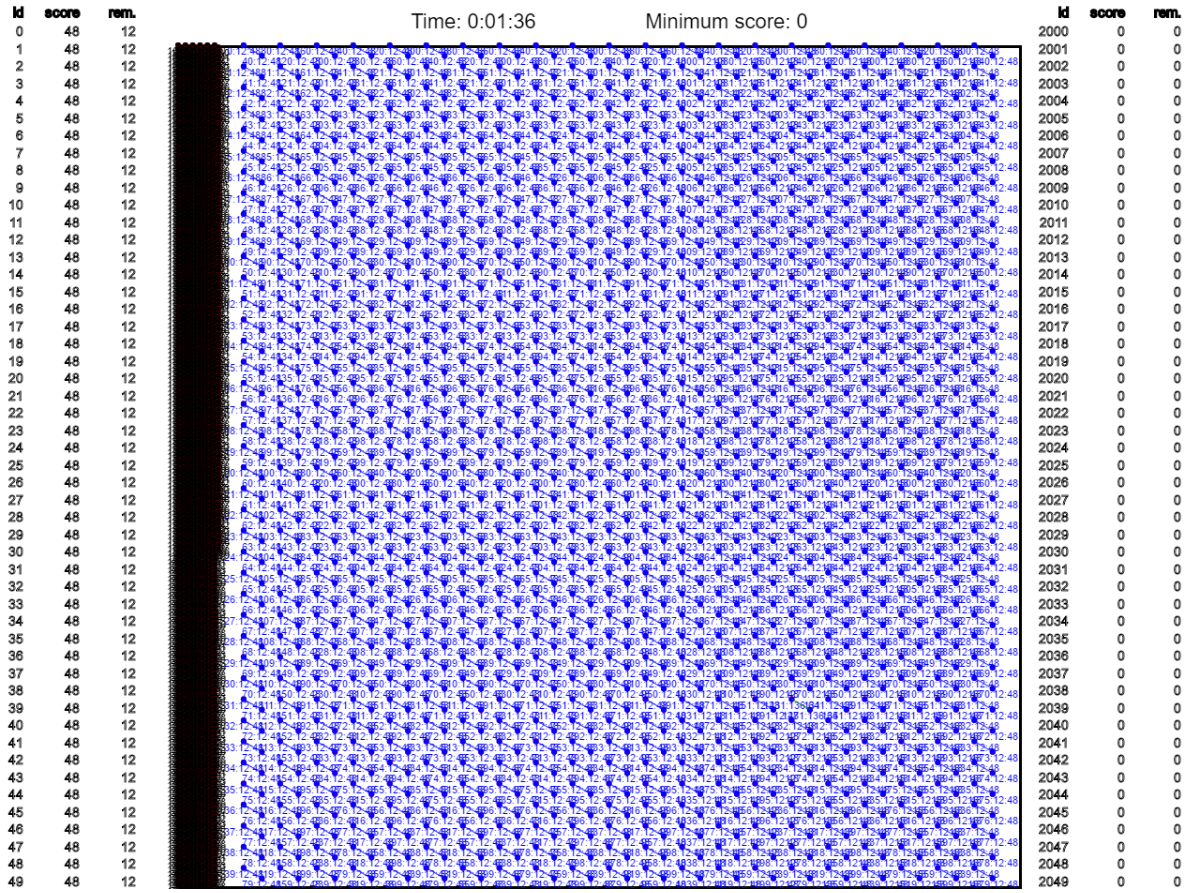
\includegraphics[width=\textwidth]{imgs/large_d_start}
\caption{Regions strategy for large values of d}
\label{large_d_start}
\end{figure}

\begin{figure} [h]
\centering
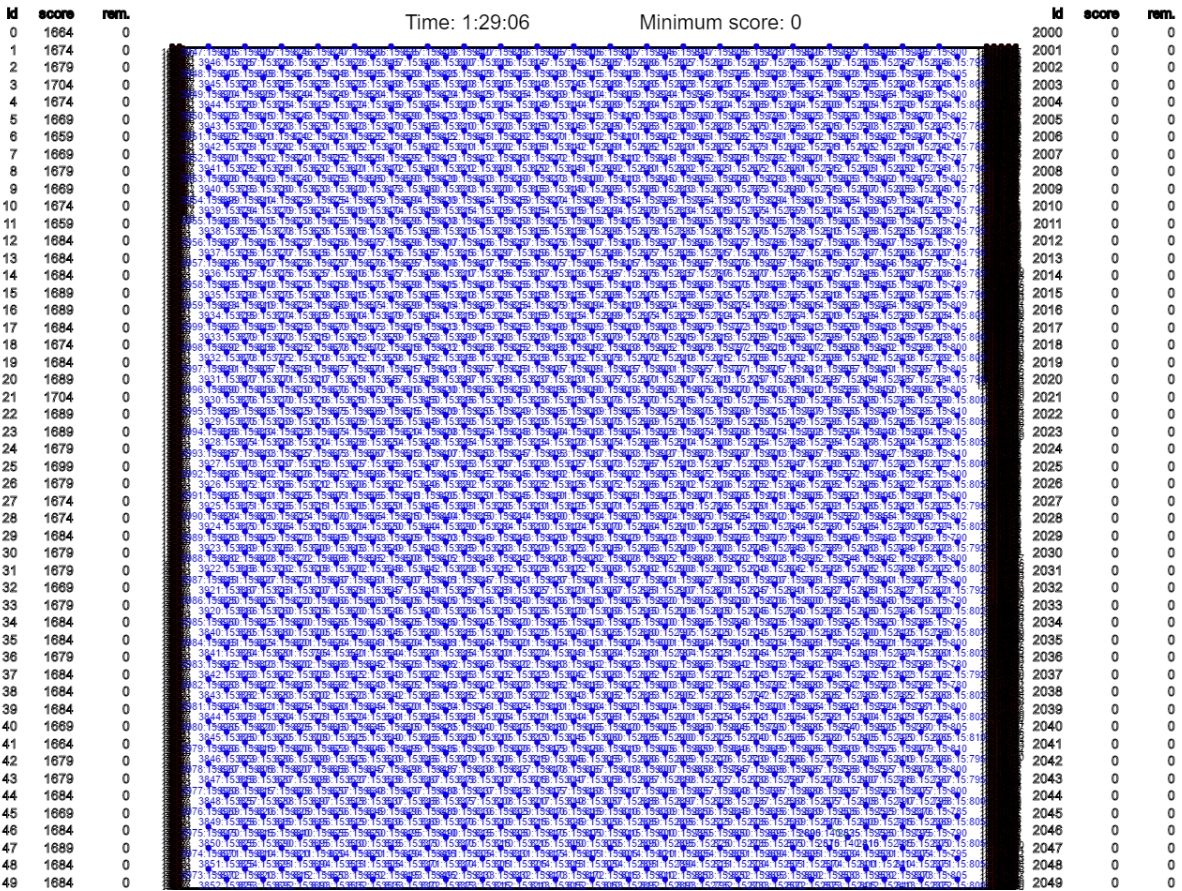
\includegraphics[width=\textwidth]{imgs/large_d_middle}
\caption{Intermediate stage for the regions strategy for large values of d}
\label{large_d_middle}
\end{figure}

\begin{figure} [h]
\centering
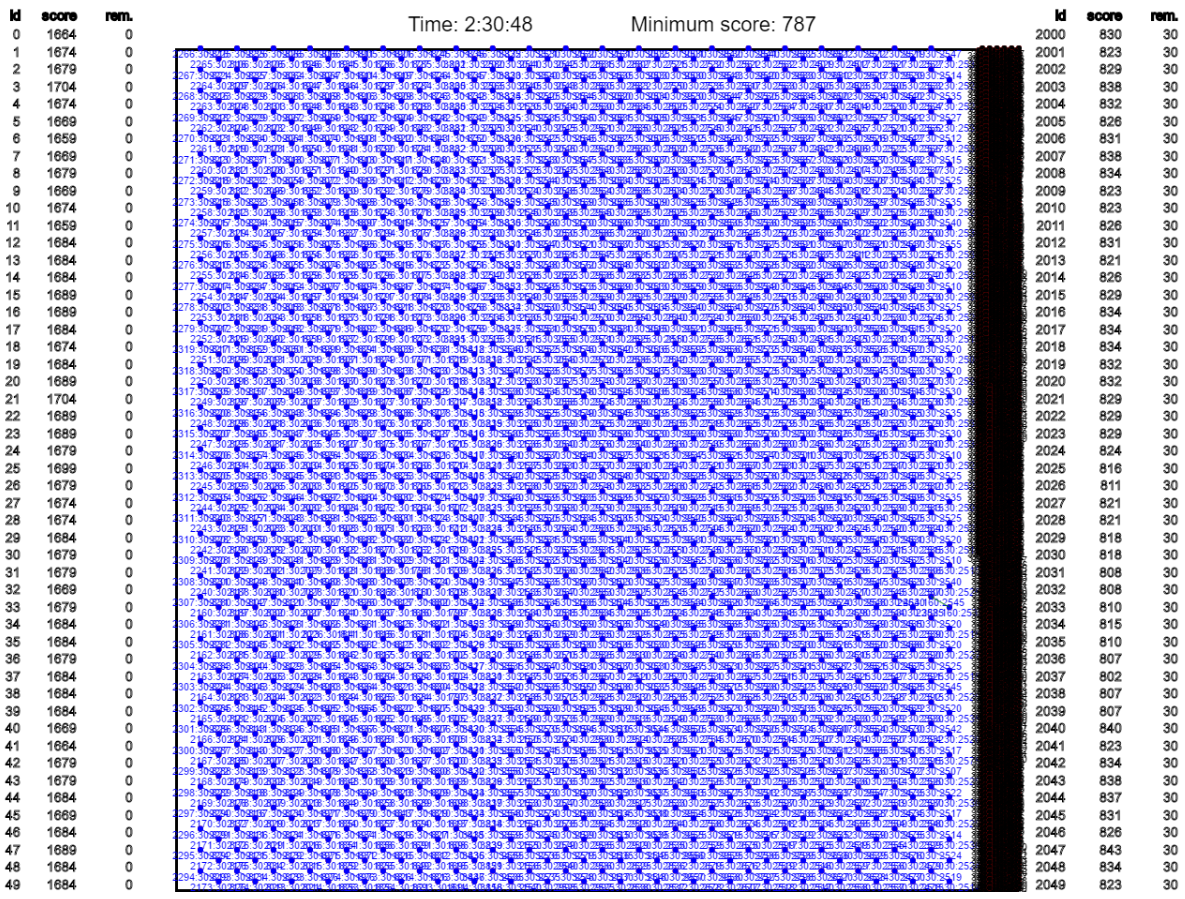
\includegraphics[width=\textwidth]{imgs/large_d_end}
\caption{Last batch in the regions strategy for large d}
\label{large_d_end}
\end{figure}

Also, each batch dances on a dance area that we also define based on d. On one side, we densely pack dancers that haven't danced yet in hexagonal columns. In the middle, we have the dancing area as a hexagonal grid of dancers, and on the other side, we have dense columns of dancers who have completed dancing in a hexagonal grid. This reduces the number of times we need to have a gap (> 0.5m) between dancers and non-dancers when compared to the conveyor strategy. \autoref{large_d_start} shows the initial configuration of the dance floor with some people on the dance floor and the rest in the left region. \autoref{large_d_middle} shows an intermediate state of the simulation where one batch has finished dancing and moved to the right, and the next batch has come to take it's place.\autoref{large_d_end} shows the last batch dancing in the center along with some of the dancers of the second last batch since the last batch may not fill the entire space, so that the dancing area is still occupied (no harm in letting people dance if we have some space left) The people who have completed dancing move to the rightmost region. This kind of strategy represents a natural kind of queuing system where lots of people arrive to dance, and wait for their turn. The dance caller decides how long each person can dance based on how much time there is and how many people there are, and makes calls in a way that he is able to provide everyone with an even amount of dancing time.

In this way, we optimize the total score that we can get, and are also able to distribute this score evenly across all dancers.

We had also debated on having the same structure over the board, and dancers moving in and out of the dancing area, or moving closer to and farther from the edges based on how high or low a dancer's score is compared to the lowest, but ruled it out because of it's similarity to group 6's strategy and it's inadequacies.

We now discuss how we calculated the size of the dancing area, how we split dancers into batches and calculated the target score. We use a gap of $0.6m$ between the dancing and non-dancing areas, so we have 18.8m left to arrange dancers. Hexagonal packing helps better our efficiency at doing this. In the idle region, we use a gap of $0.1 + \epsilon m$ between dancers, and are able to pack 200 in a column. The distance between columns in this region is $\frac{\sqrt{3}}{2} \times 0.1$, and the total width used by the idle regions is $$\frac{d-d'}{200} \times \frac{\sqrt{3}}{2} \times 0.1$$ where $d'$ is the number of dancers in a batch. Similarly, in the dancing region we pack $40$ dancers per column and the distance between columns is $\frac{\sqrt{3}}{2} \times 0.5$ and the width of this region is $$\frac{d'}{40} \times \frac{\sqrt{3}}{2} \times 0.5$$. We now get the equation $$ 18.8 = \frac{d-d'}{200} \times \frac{\sqrt{3}}{2} \times 0.1 + \frac{d'}{40} \times \frac{\sqrt{3}}{2} \times 0.5$$ We solve this equation for $d'$ to calculate the size of the dancing batch, and the number of batches is $$N = \ceil{\frac{d}{d'}}.$$

We define the target score for dancers by $S$. The number of turns it takes a dancer to reach this score using the dance-for-2-min-and-move strategy is $\frac{21 \times S}{20 \times 3}$. Assuming it takes us 9 turns for moving a batch from the idle region to the dancing region, it takes $\frac{21 \times S}{20 \times 3} + 9$ turns for a batch to reach the target score. This assumes that there is no claustrophobia while moving, but we address this detail later on when we discuss parameter tuning. Now that we know how many turns it takes for a batch to reach the score $S$, we have the equation $$ \left( \frac{21 \times S}{20 \times 3} + 9\right) \times N = 1800 $$ We know the value of $N$ and can solve for $S$. To overcome inaccuracies, we set the target score to be a percentage of this target score, which we discuss in parameter tuning.

Once we have these these values calculated, it is straightforward to implement the strategy to revolve around moving batches from the leftmost region to the dancing region to the rightmost region when all the dancers in the dancing region reach the target score.

\end{document}